\documentclass[10pt,xcolor=pdflatex,notes]{beamer}
\usepackage{newcent}
\usepackage[utf8]{inputenc}
%\usepackage[czech]{babel}
\usepackage{biblatex}
\usepackage{hyperref}
\usepackage{fancyvrb}
\usepackage{cleveref}
\usepackage{tikz}
\usepackage{tikz-qtree}
\usepackage{float}
\usepackage{xcolor}
\usepackage{listings}
\usepackage{animate}
\usepackage[linesnumbered,algoruled,boxed,lined]{algorithm2e}
% \usepackage[obeyFinal]{todonotes}

\usetikzlibrary{arrows,backgrounds,shadows, positioning}
\bibliography{bibliography.bib}


\usetheme{FIT}

\pgfdeclarelayer{edgelayer}
    \pgfdeclarelayer{nodelayer}
% tell TikZ how to stack them (back to front)
    \pgfsetlayers{nodelayer,main,edgelayer}

%%%%%%%%%%%%%%%%%%%%%%%%%%%%%%%%%%%%%%%%%%%%%%%%%%%%%%%%%%%%%%%%%%
\title[ITT - strace2seccomp]{Automatic Seccomp Syscall Policy Generator}

\author[]{Marek Tama\v{s}kovi\v{c}}

\institute[]{Brno University of Technology, Faculty of Information Technology\\
Bo\v{z}et\v{e}chova 1/2. 612 66 Brno - Kr\'alovo Pole\\
xtamas01@stud.fit.vutbr.cz}

\date{January 30, 2016}
%\date{\today}
%\date{} % bez data

%%%%%%%%%%%%%%%%%%%%%%%%%%%%%%%%%%%%%%%%%%%%%%%%%%%%%%%%%%%%%%%%%%

\begin{document}

\frame[plain]{\titlepage}

\begin{frame}\frametitle{Good News Everyone!}
	\includegraphics[width=\textwidth]{img/GoodNewsEveryone}
	\note{
	Dobry den, moje meno je XY a prisiel som vam odprezentovat moj semestralny projekt.
	}
\end{frame}

\begin{frame}\frametitle{Introduction}
	\begin{columns}
		\begin{column}{0.5\textwidth}
			\begin{itemize}
				\item What is my project?\\
				\item Why is it important?\\
			\end{itemize}
		\end{column}
		\begin{column}{0.5\textwidth}
			% \animategraphics[loop,controls,autoplay,width=\linewidth]{12}{img/purpose-}{0}{29}
			\includegraphics[width=\textwidth]{img/purpose-5}
		\end{column}
	\end{columns}
	\note{
		Co je teda moj projet? Nazov projektu je velmi vystizny a teda nazov strace2seccomp.\\
		Ako nazov napoveda projekt transformuje strace do seccomp politiky.\\
		Seccomp - secure computing je kernel modul ktory filtruje systemove volania.\\
		V zaklade po spusteni dovoli iba 4 a to read write exit a sigret.\\
		da sa rozsirit pomocou bpf filtru.\\
		Preco je to dolezite a aky to ma vyznam?\\
		Mozem obmedzit program iba na surove minimum systemovych volani. (napr. zakazem exec())\\
		Dalsia vrstva ochrana pred zneuzitim pristupu.
	}
\end{frame}

\begin{frame}\frametitle{Input / Output}
	\begin{itemize}
		\item Input
		\begin{itemize}
			\item analysis of syscall monitoring tools.
			\item used \texttt{strace}
		\end{itemize}

		\item Output
		\begin{itemize}
			\item C code (\emph{libseccomp}\footnote{https://github.com/seccomp/libseccomp})
			\item berkley packet filter
		\end{itemize}
	\end{itemize}
	\note{
		Na zaciatok takehoto projektu je treba definovat vstupy a vystupy.\\
		Po analyze asi 8 nastrojov na monitorovanie syscallov som sa rozhodol pouzit strace <- EZ2use.\\
		Na vystup boli dve moznosti. \\
		Surovy bpf filter. vela moznosti ako nastavit avsak prilis narocne.\\
		libseccomp c wrapper nad bpf. Jednoduchy na pouzitie, <- moja volba.
	}
\end{frame}

\begin{frame}\frametitle{Architecture}
	\begin{figure}[h]
		\centering
		\resizebox {\textwidth} {!} {
			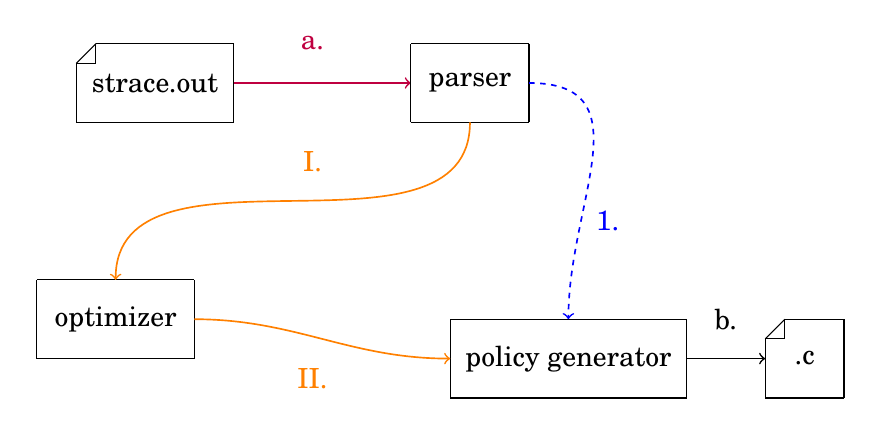
\begin{tikzpicture}
	\begin{pgfonlayer}{nodelayer}
		\node [] (0) at (-6.75, 6) {};
		\node [] (1) at (-6.75, 5) {};
		\node [] (2) at (-8.75, 5) {};
		\node [] (3) at (-6.75, 5.5) {};
		\node [] (4) at (-4.5, 5.5) {};
		\node [] (5) at (-4.5, 6) {};
		\node [] (6) at (-4.5, 5) {};
		\node [] (7) at (-3, 5) {};
		\node [] (8) at (-3, 6) {};
		\node [] (9) at (-9.25, 3) {};
		\node [] (10) at (-7.25, 3) {};
		\node [] (11) at (-7.25, 2) {};
		\node [] (12) at (-9.25, 2) {};
		\node [] (13) at (-8.25, 2.5) {optimizer};
		\node [] (14) at (-4, 2.5) {};
		\node [] (15) at (-4, 1.5) {};
		\node [] (16) at (-1, 2.5) {};
		\node [] (17) at (-1, 1.5) {};
		\node [] (18) at (-2.5, 2) {policy generator};
		\node [] (19) at (-2.5, 2.5) {};
		\node [] (20) at (-4, 2) {};
		\node [] (21) at (-3.75, 5) {};
		\node [] (22) at (-8.25, 3) {};
		\node [] (23) at (-7.25, 2.5) {};
		\node [] (24) at (-3, 5.5) {};
		\node [] (25) at (-7.75, 5.5) {strace.out};
		\node [] (26) at (0, 1.5) {};
		\node [] (27) at (1, 1.5) {};
		\node [] (28) at (1, 2.5) {};
		\node [] (29) at (0.5, 2) {.c};
		\node [] (30) at (0, 2) {};
		\node [] (31) at (-1, 2) {};
		\node [] (32) at (-3.75, 5.5) {parser};
		\node [style={color=blue}] (33) at (-2, 3.75) {1.};
		\node [style={color=purple}] (34) at (-5.75, 6) {a.};
		\node [style={color=orange}] (35) at (-5.75, 4.5) {I.};
		\node [style={color=orange}] (36) at (-5.75, 1.75) {II.};
		\node [] (37) at (0, 2.25) {};
		\node [] (38) at (0.25, 2.5) {};
		\node [] (39) at (-8.75, 5.75) {};
		\node [] (40) at (-8.5, 6) {};
		\node [] (41) at (0.25, 2.25) {};
		\node [] (42) at (-8.5, 5.75) {};
		\node [] (43) at (-0.5, 2.5) {b.};
	\end{pgfonlayer}
	\begin{pgfonlayer}{edgelayer}
		\draw (20.center) to (15.center);
		\draw (15.center) to (17.center);
		\draw (16.center) to (19.center);
		\draw (19.center) to (14.center);
		\draw (14.center) to (20.center);
		\draw (11.center) to (12.center);
		\draw (12.center) to (9.center);
		\draw (2.center) to (1.center);
		\draw (1.center) to (3.center);
		\draw (3.center) to (0.center);
		\draw [semithick, color=purple, ->] (3.center) to (4.center);
		\draw (4.center) to (5.center);
		\draw (5.center) to (8.center);
		\draw (6.center) to (4.center);
		\draw (6.center) to (21.center);
		\draw (21.center) to (7.center);
		\draw (9.center) to (22.center);
		\draw (22.center) to (10.center);
		\draw [semithick, color=orange, <-, in=-90, out=90, looseness=1.00] (22.center) to (21.center);
		\draw (10.center) to (23.center);
		\draw (23.center) to (11.center);
		\draw [semithick, color=orange, ->, in=180, out=0, looseness=1.00] (23.center) to (20.center);
		\draw (8.center) to (24.center);
		\draw (24.center) to (7.center);
		\draw [semithick, color=blue, dash pattern=on 2pt off 2pt, ->, in=90, out=0, looseness=1.25] (24.center) to (19.center);
		\draw (28.center) to (27.center);
		\draw (27.center) to (26.center);
		\draw (30.center) to (26.center);
		\draw (16.center) to (31.center);
		\draw (31.center) to (17.center);
		\draw [semithick, ->] (31.center) to (30.center);
		\draw (40.center) to (39.center);
		\draw (39.center) to (2.center);
		\draw (40.center) to (0.center);
		\draw (38.center) to (37.center);
		\draw (37.center) to (30.center);
		\draw (38.center) to (28.center);
		\draw (38.center) to (41.center);
		\draw (37.center) to (41.center);
		\draw (40.center) to (42.center);
		\draw (42.center) to (39.center);
	\end{pgfonlayer}
\end{tikzpicture}

		}
		% \caption{Architecture of strace2seccomp}
		\label{fig:tikz:architecture}
	\end{figure}
	\note{
		Na tomto obrazku mozte vidiet architektura programu.\\
		Pouzil som architekturny vzor Pipe\&Filter. Inspiracia z prekladacov\\
		Sklada sa zo 3 casti.\\
	}
\end{frame}


\begin{frame}\frametitle{Processing}
	\begin{itemize}
		\item parser
		\item intermediate data structure
		\item optimizer (algorithms)
		\begin{itemize}
			\item strict
			\item weak
			\item advanced
		\end{itemize}
		\item output generator
	\end{itemize}
	\note{
		Parser (PEGTL).\\
		IDS - ukazem na dalsom slide\\
		Translator - prelozi IDS do .c\\
		Optimizer - 3 algortimy Strict, Weak, Advanced\\
		Strict - prelozi 1:1\\
		Weak - vyhlada extremy a to pouzije ako hranice intervalu.
		Advanced kombinacia oboch. Pri urcitom pocte vyskitu argumentov sa zachova na roznych vrstvach inak.
	}
\end{frame}

\begin{frame}
	\frametitle{IDS - tree}
	\begin{figure}[h]
\centering
  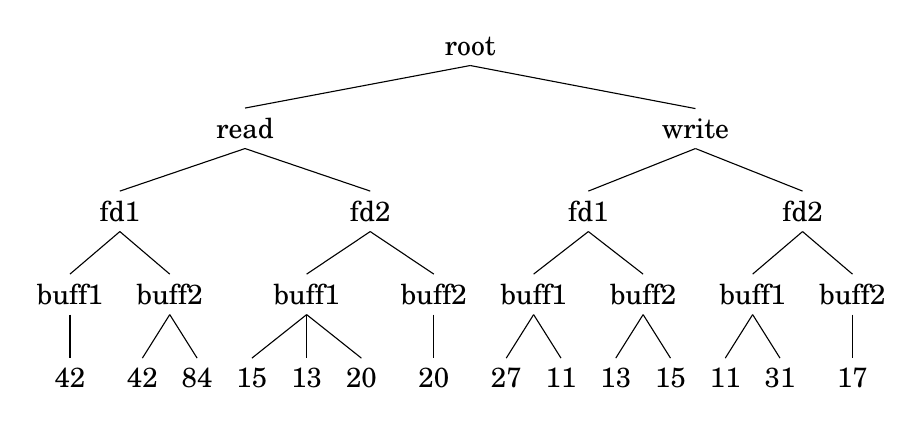
\begin{tikzpicture}
  \Tree [.root
          [.read
            [.fd1
              [.buff1 42 ]
              [.buff2 42 84 ]
            ]
            [.fd2
              [.buff1 15 13 20 ]
              [.buff2 20 ]
            ]
          ]
          [.write
            [.fd1
              [.buff1 27 11 ]
              [.buff2 13 15 ]
            ]
            [.fd2
              [.buff1 11 31 ]
              [.buff2 17 ]
            ]
          ]
        ]
  \end{tikzpicture}
  % \caption{Visualized IDS as a tree}
  \label{fig:tikz:IDStree}
\end{figure}
	\note{Ukazka stromu IDS}
\end{frame}

\begin{frame}\frametitle{What have I done?}
	\begin{itemize}
		\item syscall monitoring tools analysis
		\item requirements definition
		\item design architecture
		\item design algorithms to process IDS\footnote{Intermediate Data Structure}
	\end{itemize}
	\note{Spomenute + Statitika: 16 normostran textu.}
\end{frame}

\begin{frame}\frametitle{What am I planning to do?}
	\begin{itemize}
		\item{Implementation}
		\begin{itemize}
			\item 3 algorithm specified earlier
			\item \textit{translation direct to BPF}
		\end{itemize}
		\item{Testing}
		\begin{itemize}
			\item parser fuzzy testing\cite{fuzzy}
			\item on real project (\textit{usbguard}\footnote{https://usbguard.github.io/}).
		\end{itemize}
		\item{Documentation}
		\begin{itemize}
			\item finish text in bachelor thesis
			\item document source code
			\item make manual how to use it
		\end{itemize}
	\end{itemize}
	\note{
		Implementacia - priamo to co je popisane + autotools / cmake
		Testovanie - otestova t to na realnom produkte ci to je funkcne ci nebude nasilne ukonceny apod.
		fuzzying nad parserom - overenie funkcnosti a stability.
		Dokumentacia - samozreme je treba dokoncit BP
		-taktiez treba popisat ako sa to pouziva spravit manual
		-dokumentacia zdrojakov je samozrejmost
	}
\end{frame}

\bluepage{Thank You For Your Attention !}

\begin{frame}\frametitle{Apendix - 1}
	\begin{figure}[h]
		\centering
		\resizebox {\textwidth} {!} {
			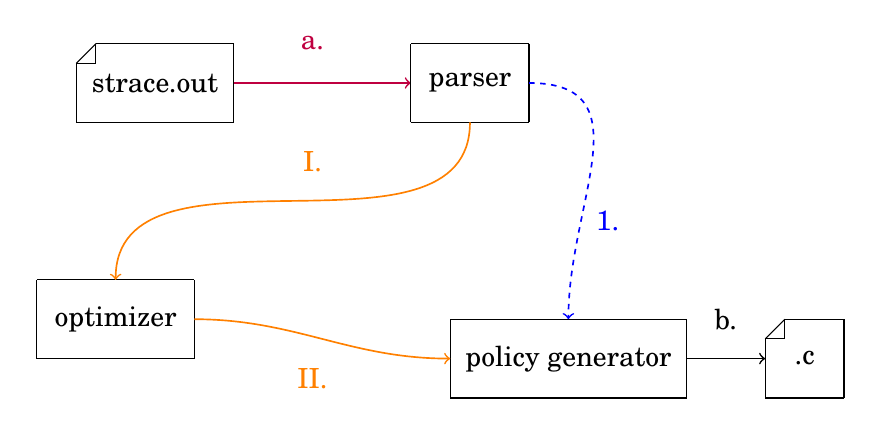
\begin{tikzpicture}
	\begin{pgfonlayer}{nodelayer}
		\node [] (0) at (-6.75, 6) {};
		\node [] (1) at (-6.75, 5) {};
		\node [] (2) at (-8.75, 5) {};
		\node [] (3) at (-6.75, 5.5) {};
		\node [] (4) at (-4.5, 5.5) {};
		\node [] (5) at (-4.5, 6) {};
		\node [] (6) at (-4.5, 5) {};
		\node [] (7) at (-3, 5) {};
		\node [] (8) at (-3, 6) {};
		\node [] (9) at (-9.25, 3) {};
		\node [] (10) at (-7.25, 3) {};
		\node [] (11) at (-7.25, 2) {};
		\node [] (12) at (-9.25, 2) {};
		\node [] (13) at (-8.25, 2.5) {optimizer};
		\node [] (14) at (-4, 2.5) {};
		\node [] (15) at (-4, 1.5) {};
		\node [] (16) at (-1, 2.5) {};
		\node [] (17) at (-1, 1.5) {};
		\node [] (18) at (-2.5, 2) {policy generator};
		\node [] (19) at (-2.5, 2.5) {};
		\node [] (20) at (-4, 2) {};
		\node [] (21) at (-3.75, 5) {};
		\node [] (22) at (-8.25, 3) {};
		\node [] (23) at (-7.25, 2.5) {};
		\node [] (24) at (-3, 5.5) {};
		\node [] (25) at (-7.75, 5.5) {strace.out};
		\node [] (26) at (0, 1.5) {};
		\node [] (27) at (1, 1.5) {};
		\node [] (28) at (1, 2.5) {};
		\node [] (29) at (0.5, 2) {.c};
		\node [] (30) at (0, 2) {};
		\node [] (31) at (-1, 2) {};
		\node [] (32) at (-3.75, 5.5) {parser};
		\node [style={color=blue}] (33) at (-2, 3.75) {1.};
		\node [style={color=purple}] (34) at (-5.75, 6) {a.};
		\node [style={color=orange}] (35) at (-5.75, 4.5) {I.};
		\node [style={color=orange}] (36) at (-5.75, 1.75) {II.};
		\node [] (37) at (0, 2.25) {};
		\node [] (38) at (0.25, 2.5) {};
		\node [] (39) at (-8.75, 5.75) {};
		\node [] (40) at (-8.5, 6) {};
		\node [] (41) at (0.25, 2.25) {};
		\node [] (42) at (-8.5, 5.75) {};
		\node [] (43) at (-0.5, 2.5) {b.};
	\end{pgfonlayer}
	\begin{pgfonlayer}{edgelayer}
		\draw (20.center) to (15.center);
		\draw (15.center) to (17.center);
		\draw (16.center) to (19.center);
		\draw (19.center) to (14.center);
		\draw (14.center) to (20.center);
		\draw (11.center) to (12.center);
		\draw (12.center) to (9.center);
		\draw (2.center) to (1.center);
		\draw (1.center) to (3.center);
		\draw (3.center) to (0.center);
		\draw [semithick, color=purple, ->] (3.center) to (4.center);
		\draw (4.center) to (5.center);
		\draw (5.center) to (8.center);
		\draw (6.center) to (4.center);
		\draw (6.center) to (21.center);
		\draw (21.center) to (7.center);
		\draw (9.center) to (22.center);
		\draw (22.center) to (10.center);
		\draw [semithick, color=orange, <-, in=-90, out=90, looseness=1.00] (22.center) to (21.center);
		\draw (10.center) to (23.center);
		\draw (23.center) to (11.center);
		\draw [semithick, color=orange, ->, in=180, out=0, looseness=1.00] (23.center) to (20.center);
		\draw (8.center) to (24.center);
		\draw (24.center) to (7.center);
		\draw [semithick, color=blue, dash pattern=on 2pt off 2pt, ->, in=90, out=0, looseness=1.25] (24.center) to (19.center);
		\draw (28.center) to (27.center);
		\draw (27.center) to (26.center);
		\draw (30.center) to (26.center);
		\draw (16.center) to (31.center);
		\draw (31.center) to (17.center);
		\draw [semithick, ->] (31.center) to (30.center);
		\draw (40.center) to (39.center);
		\draw (39.center) to (2.center);
		\draw (40.center) to (0.center);
		\draw (38.center) to (37.center);
		\draw (37.center) to (30.center);
		\draw (38.center) to (28.center);
		\draw (38.center) to (41.center);
		\draw (37.center) to (41.center);
		\draw (40.center) to (42.center);
		\draw (42.center) to (39.center);
	\end{pgfonlayer}
\end{tikzpicture}

		}
		% \caption{Architecture}
		\label{fig:tikz:architecture2}
	\end{figure}
\end{frame}

\begin{frame}\frametitle{Apendix - 2}
\begin{center}
\scalebox{.8}{
	\begin{algorithm}[H]
		\SetKwData{syscall}{sc}
		\SetKwData{ids}{IDS}
		\SetKwData{argument}{arg}
		\SetKwData{level}{lvl}
		\SetKwData{numArgs}{num\_arg}
		\SetKwData{intervals}{intervals}
		\SetKwData{rules}{rules}

		\SetKwFunction{GetNumArgs}{get\_num\_args}
		\SetKwFunction{Append}{append}
		\SetKwFunction{getMinMax}{get\_minmax}

		\KwIn{intermediate data structure \ids}
		\KwOut{list of rules \rules}

		\caption{Weak optimization}\label{algo:weak}
		\ForEach{syscall \syscall in the \ids}{
			\ForEach{argument \argument in the syscall \syscall}{
				\numArgs $\leftarrow$ \GetNumArgs{p}\;
				\For{$\level \leftarrow 0$ \KwTo \numArgs}{
					\intervals.\Append{\getMinMax{\argument, \level}}\;
				}
				\rules.\Append{\syscall, \intervals}\;
			}
		}
	\end{algorithm}
}
\end{center}
\end{frame}



\begin{frame}[allowframebreaks]
	\frametitle{References}
	\printbibliography
\end{frame}
\end{document}
